% Created by tikzDevice version 0.12.3.1 on 2021-11-10 17:09:39
% !TEX encoding = UTF-8 Unicode
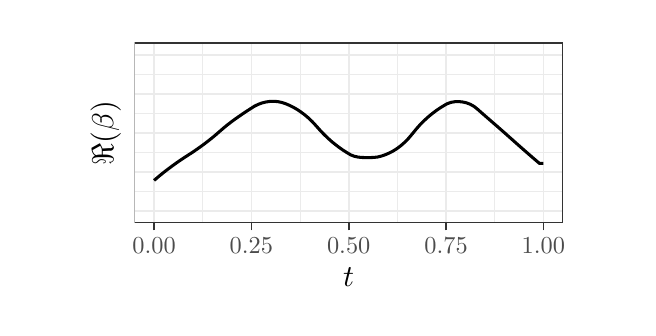
\begin{tikzpicture}[x=1pt,y=1pt]
\definecolor{fillColor}{RGB}{255,255,255}
\path[use as bounding box,fill=fillColor,fill opacity=0.00] (0,0) rectangle (216.81,101.18);
\begin{scope}
\path[clip] ( 17.93,  0.00) rectangle (198.88,101.18);
\definecolor{drawColor}{RGB}{255,255,255}
\definecolor{fillColor}{RGB}{255,255,255}

\path[draw=drawColor,line width= 0.6pt,line join=round,line cap=round,fill=fillColor] ( 17.93,  0.00) rectangle (198.88,101.18);
\end{scope}
\begin{scope}
\path[clip] ( 38.64, 30.69) rectangle (193.38, 95.68);
\definecolor{fillColor}{RGB}{255,255,255}

\path[fill=fillColor] ( 38.64, 30.69) rectangle (193.38, 95.68);
\definecolor{drawColor}{gray}{0.92}

\path[draw=drawColor,line width= 0.3pt,line join=round] ( 38.64, 42.08) --
	(193.38, 42.08);

\path[draw=drawColor,line width= 0.3pt,line join=round] ( 38.64, 56.15) --
	(193.38, 56.15);

\path[draw=drawColor,line width= 0.3pt,line join=round] ( 38.64, 70.22) --
	(193.38, 70.22);

\path[draw=drawColor,line width= 0.3pt,line join=round] ( 38.64, 84.28) --
	(193.38, 84.28);

\path[draw=drawColor,line width= 0.3pt,line join=round] ( 63.26, 30.69) --
	( 63.26, 95.68);

\path[draw=drawColor,line width= 0.3pt,line join=round] ( 98.43, 30.69) --
	( 98.43, 95.68);

\path[draw=drawColor,line width= 0.3pt,line join=round] (133.60, 30.69) --
	(133.60, 95.68);

\path[draw=drawColor,line width= 0.3pt,line join=round] (168.77, 30.69) --
	(168.77, 95.68);

\path[draw=drawColor,line width= 0.6pt,line join=round] ( 38.64, 35.05) --
	(193.38, 35.05);

\path[draw=drawColor,line width= 0.6pt,line join=round] ( 38.64, 49.11) --
	(193.38, 49.11);

\path[draw=drawColor,line width= 0.6pt,line join=round] ( 38.64, 63.18) --
	(193.38, 63.18);

\path[draw=drawColor,line width= 0.6pt,line join=round] ( 38.64, 77.25) --
	(193.38, 77.25);

\path[draw=drawColor,line width= 0.6pt,line join=round] ( 38.64, 91.32) --
	(193.38, 91.32);

\path[draw=drawColor,line width= 0.6pt,line join=round] ( 45.67, 30.69) --
	( 45.67, 95.68);

\path[draw=drawColor,line width= 0.6pt,line join=round] ( 80.84, 30.69) --
	( 80.84, 95.68);

\path[draw=drawColor,line width= 0.6pt,line join=round] (116.01, 30.69) --
	(116.01, 95.68);

\path[draw=drawColor,line width= 0.6pt,line join=round] (151.18, 30.69) --
	(151.18, 95.68);

\path[draw=drawColor,line width= 0.6pt,line join=round] (186.35, 30.69) --
	(186.35, 95.68);
\definecolor{drawColor}{RGB}{0,0,0}

\path[draw=drawColor,line width= 1.1pt,line join=round] ( 45.67, 45.98) --
	( 47.07, 47.17) --
	( 48.46, 48.32) --
	( 49.85, 49.42) --
	( 51.25, 50.48) --
	( 52.64, 51.51) --
	( 54.03, 52.50) --
	( 55.42, 53.45) --
	( 56.82, 54.38) --
	( 58.21, 55.27) --
	( 59.60, 56.18) --
	( 61.00, 57.13) --
	( 62.39, 58.11) --
	( 63.78, 59.13) --
	( 65.17, 60.19) --
	( 66.57, 61.30) --
	( 67.96, 62.46) --
	( 69.35, 63.67) --
	( 70.75, 64.88) --
	( 72.14, 66.02) --
	( 73.53, 67.09) --
	( 74.92, 68.12) --
	( 76.32, 69.10) --
	( 77.71, 70.05) --
	( 79.10, 70.98) --
	( 80.50, 71.88) --
	( 81.89, 72.77) --
	( 83.28, 73.46) --
	( 84.67, 73.97) --
	( 86.07, 74.32) --
	( 87.46, 74.52) --
	( 88.85, 74.57) --
	( 90.24, 74.47) --
	( 91.64, 74.21) --
	( 93.03, 73.77) --
	( 94.42, 73.19) --
	( 95.82, 72.51) --
	( 97.21, 71.72) --
	( 98.60, 70.81) --
	( 99.99, 69.78) --
	(101.39, 68.60) --
	(102.78, 67.28) --
	(104.17, 65.78) --
	(105.57, 64.20) --
	(106.96, 62.73) --
	(108.35, 61.38) --
	(109.74, 60.13) --
	(111.14, 58.98) --
	(112.53, 57.93) --
	(113.92, 56.95) --
	(115.32, 56.05) --
	(116.71, 55.22) --
	(118.10, 54.69) --
	(119.49, 54.40) --
	(120.89, 54.27) --
	(122.28, 54.24) --
	(123.67, 54.24) --
	(125.07, 54.29) --
	(126.46, 54.45) --
	(127.85, 54.79) --
	(129.24, 55.28) --
	(130.64, 55.87) --
	(132.03, 56.60) --
	(133.42, 57.47) --
	(134.82, 58.51) --
	(136.21, 59.74) --
	(137.60, 61.16) --
	(138.99, 62.80) --
	(140.39, 64.53) --
	(141.78, 66.10) --
	(143.17, 67.51) --
	(144.57, 68.79) --
	(145.96, 69.96) --
	(147.35, 71.02) --
	(148.74, 71.99) --
	(150.14, 72.87) --
	(151.53, 73.68) --
	(152.92, 74.18) --
	(154.31, 74.42) --
	(155.71, 74.47) --
	(157.10, 74.34) --
	(158.49, 74.04) --
	(159.89, 73.52) --
	(161.28, 72.74) --
	(162.67, 71.62) --
	(164.06, 70.39) --
	(165.46, 69.17) --
	(166.85, 67.96) --
	(168.24, 66.75) --
	(169.64, 65.54) --
	(171.03, 64.32) --
	(172.42, 63.10) --
	(173.81, 61.86) --
	(175.21, 60.62) --
	(176.60, 59.38) --
	(177.99, 58.15) --
	(179.39, 56.92) --
	(180.78, 55.71) --
	(182.17, 54.50) --
	(183.56, 53.30) --
	(184.96, 52.11) --
	(186.35, 52.11);
\definecolor{drawColor}{gray}{0.20}

\path[draw=drawColor,line width= 0.6pt,line join=round,line cap=round] ( 38.64, 30.69) rectangle (193.38, 95.68);
\end{scope}
\begin{scope}
\path[clip] (  0.00,  0.00) rectangle (216.81,101.18);
\definecolor{drawColor}{gray}{0.20}

\path[draw=drawColor,line width= 0.6pt,line join=round] ( 45.67, 27.94) --
	( 45.67, 30.69);

\path[draw=drawColor,line width= 0.6pt,line join=round] ( 80.84, 27.94) --
	( 80.84, 30.69);

\path[draw=drawColor,line width= 0.6pt,line join=round] (116.01, 27.94) --
	(116.01, 30.69);

\path[draw=drawColor,line width= 0.6pt,line join=round] (151.18, 27.94) --
	(151.18, 30.69);

\path[draw=drawColor,line width= 0.6pt,line join=round] (186.35, 27.94) --
	(186.35, 30.69);
\end{scope}
\begin{scope}
\path[clip] (  0.00,  0.00) rectangle (216.81,101.18);
\definecolor{drawColor}{gray}{0.30}

\node[text=drawColor,anchor=base,inner sep=0pt, outer sep=0pt, scale=  0.88] at ( 45.67, 19.68) {0.00};

\node[text=drawColor,anchor=base,inner sep=0pt, outer sep=0pt, scale=  0.88] at ( 80.84, 19.68) {0.25};

\node[text=drawColor,anchor=base,inner sep=0pt, outer sep=0pt, scale=  0.88] at (116.01, 19.68) {0.50};

\node[text=drawColor,anchor=base,inner sep=0pt, outer sep=0pt, scale=  0.88] at (151.18, 19.68) {0.75};

\node[text=drawColor,anchor=base,inner sep=0pt, outer sep=0pt, scale=  0.88] at (186.35, 19.68) {1.00};
\end{scope}
\begin{scope}
\path[clip] (  0.00,  0.00) rectangle (216.81,101.18);
\definecolor{drawColor}{RGB}{0,0,0}

\node[text=drawColor,anchor=base,inner sep=0pt, outer sep=0pt, scale=  1.10] at (116.01,  7.64) {$t$};
\end{scope}
\begin{scope}
\path[clip] (  0.00,  0.00) rectangle (216.81,101.18);
\definecolor{drawColor}{RGB}{0,0,0}

\node[text=drawColor,rotate= 90.00,anchor=base,inner sep=0pt, outer sep=0pt, scale=  1.10] at ( 31.00, 63.18) {$\Re(\beta)$};
\end{scope}
\end{tikzpicture}
